% % 插入图片的模板,只需要修改width和图片名
% \begin{figure}[htb]
%     \centering
%     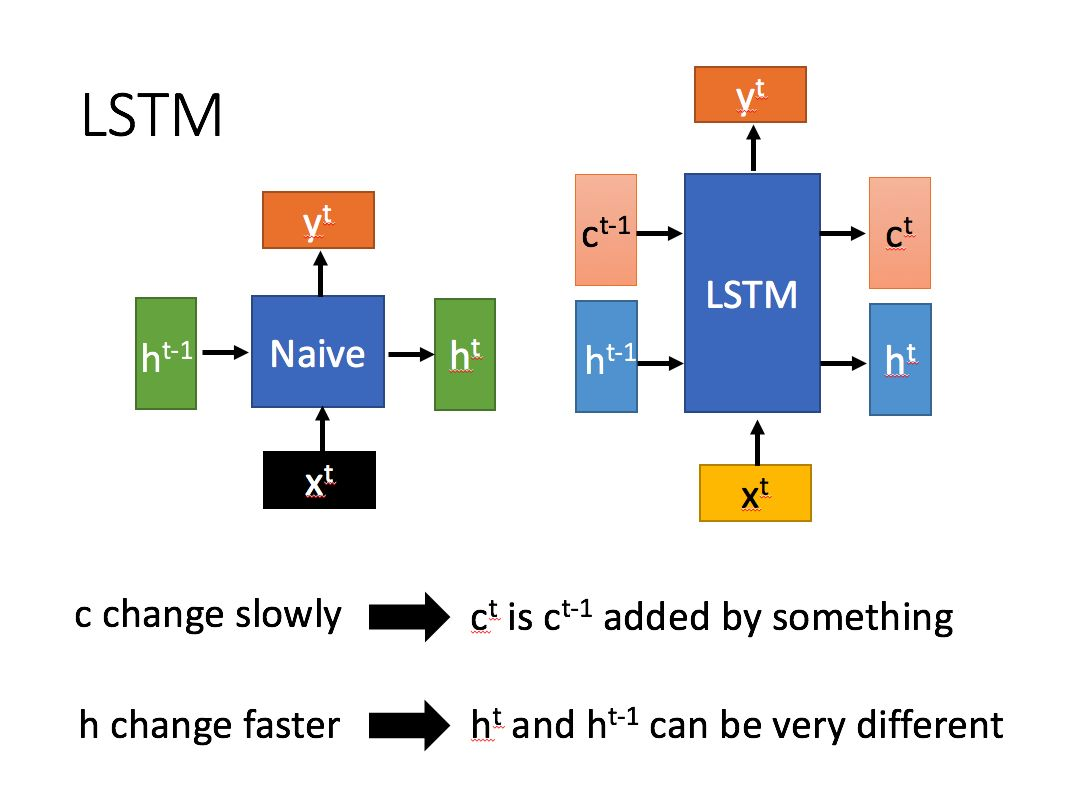
\includegraphics[width = 0.8\textwidth]{fig/LSTM1.jpg}  % 占文本可用宽度的0.8
%     \caption{Modeling framework}
%     \label{fig:framework}
% \end{figure}

% % 插入2子图的模板,用subfigure{}函数
% \begin{figure}[htb]
% \centering
% \subfigure[Before smooth]{
% 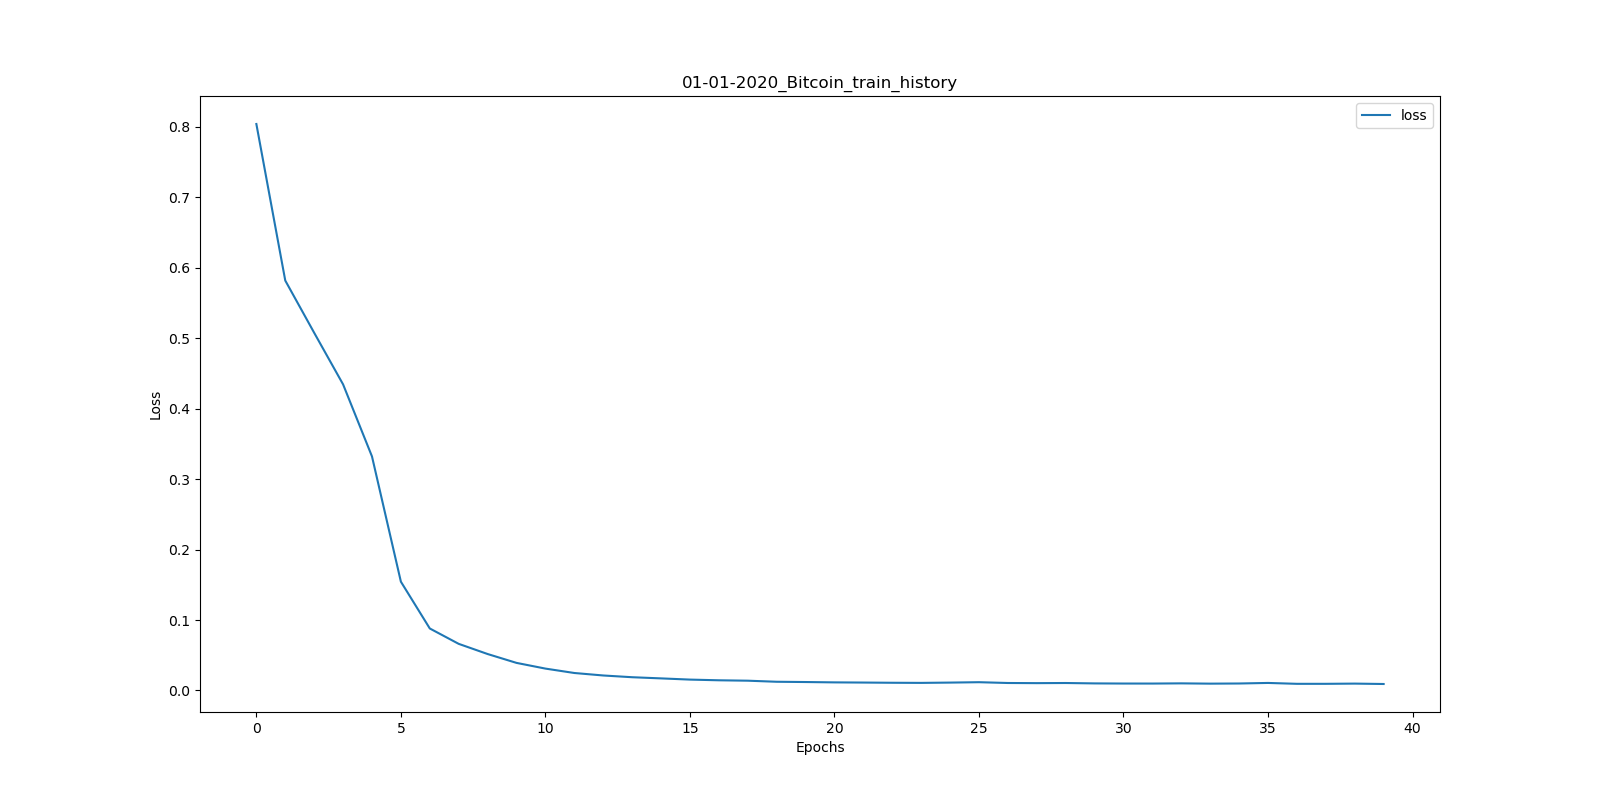
\includegraphics[width = 4.5in]{fig/convergence speed of training loss before smooth.png}
% \label{before smooth}
% }
% \subfigure[After smooth]{
% 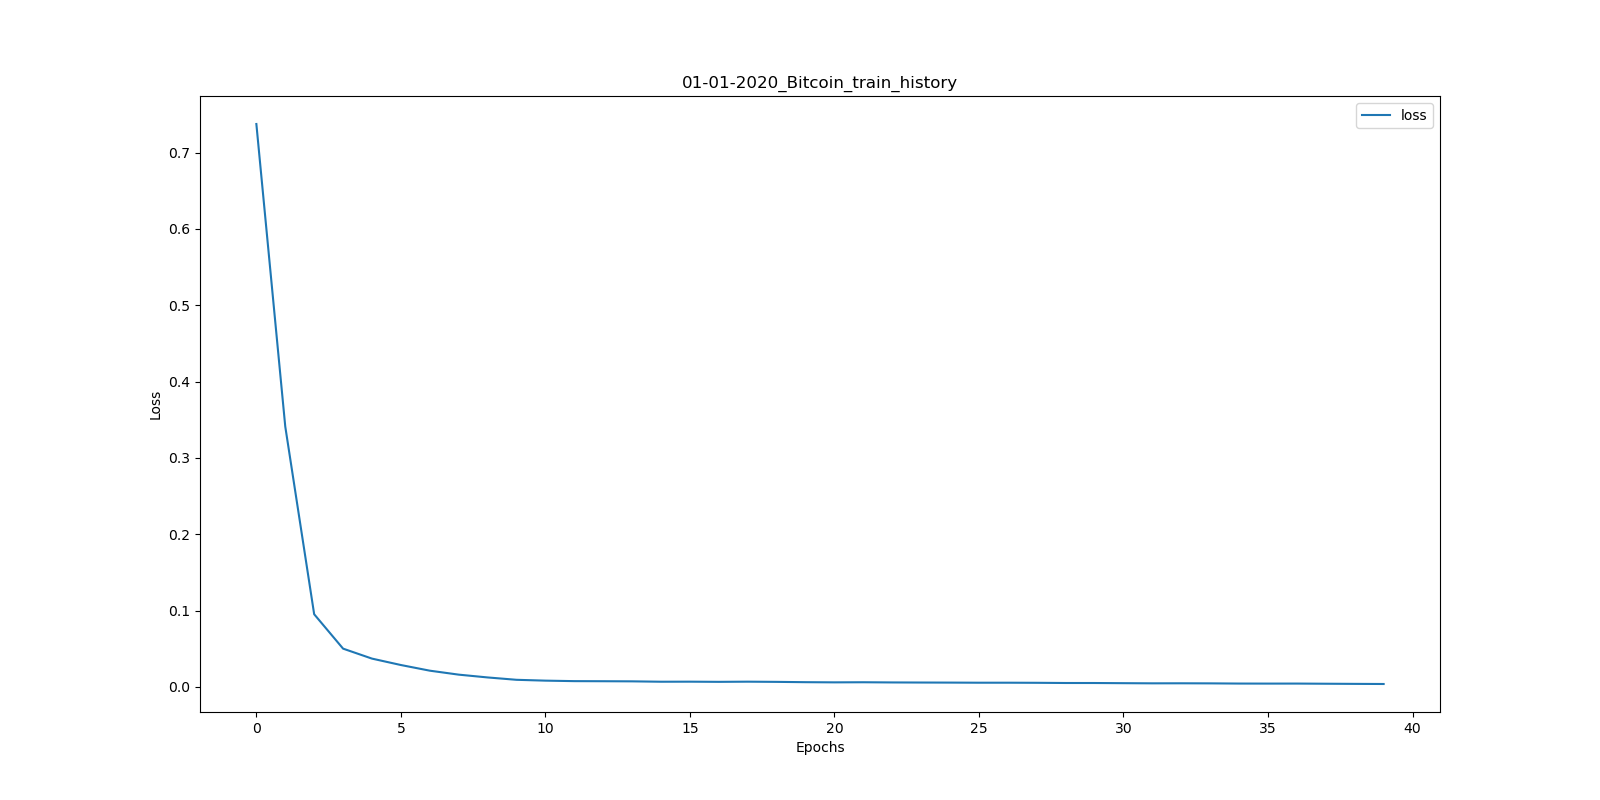
\includegraphics[width = 4.5in]{fig/convergence speed of training loss after smooth.png}
% \label{after smooth}
% }
% \caption{Contrast regarding smooth method}
% \label{fig:smooth}
% \end{figure}